%%%%%%%%%%%%%%%%%%%%%%%%%%%%%%%%%%%%
% Lesson Plan (50 minutes)
%%%%%%%%%%%%%%%%%%%%%%%%%%%%%%%%%%%%
\begin{frame}
    \frametitle{Lesson Plan}
    \begin{itemize}
        \item xx min Lecture: Continuous distributions, probability density functions
        \item xx min R Demonstration: Continuous distribution examples
        \item xx min Edfinity quiz: concepts
        % TODO: will need to fill in a lot of the material in this lecture
    \end{itemize}
\end{frame}

%%%%%%%%%%%%%%%%%%%%%%%%%%%%%%%%%%%%
% Learning objectives:
%%%%%%%%%%%%%%%%%%%%%%%%%%%%%%%%%%%%
\begin{frame}
    \frametitle{Learning Objectives}
    \begin{itemize}
        \item \textbf{M1 LO3: Use R for Data Management and Exploration:} Utilize R to load, pre-process, and explore data through visualization and summarization techniques.
        \item \textbf{M6 LO1: Validate and Explain Probability Distributions:} Assess the validity of a probability distribution using the concepts of outcome, sample space, and probability properties (e.g., disjoint outcomes, probabilities between 0 and 1, and total probabilities summing to 1).
        \item \textbf{M6 LO3: Compute Probabilities Using Various Tools:} Use logic, Venn diagrams, and probability rules to compute probabilities for events.
        \item \textbf{M6 LO4: Understand and Compute Expectations and Variances:} Explain the concepts of expectations and variances of random variables, and compute the expectation and variance of a linear combination of random variables.
        \item \textbf{M6 LO6: Assess Data Using the Normal Distribution:} Use the normal distribution to assess the "unusualness" of data points, apply the 68-95-99.7% rule, evaluate normality through histograms and q-q plots, and determine when a normal approximation to the binomial model is valid for calculating binomial probabilities.
    \end{itemize}
\end{frame}

%%%%%%%%%%%%%%%%%%%%%%%%%%%%%%%%%%%%
% TODO: Copy and adapt these slides base on the lesson plan
%%%%%%%%%%%%%%%%%%%%%%%%%%%%%%%%%%%%

\section{Continuous distributions}

%%%%%%%%%%%%%%%%%%%%%%%%%%%%%%%%%%%%

\begin{frame}
\frametitle{Continuous distributions}

\begin{itemize}

\item Below is a histogram of the distribution of heights of US adults. 

\item The proportion of data that falls in the shaded bins gives the probability that a randomly sampled US adult is between 180 cm and 185 cm (about 5'11" to 6'1").

\end{itemize}

\begin{center}
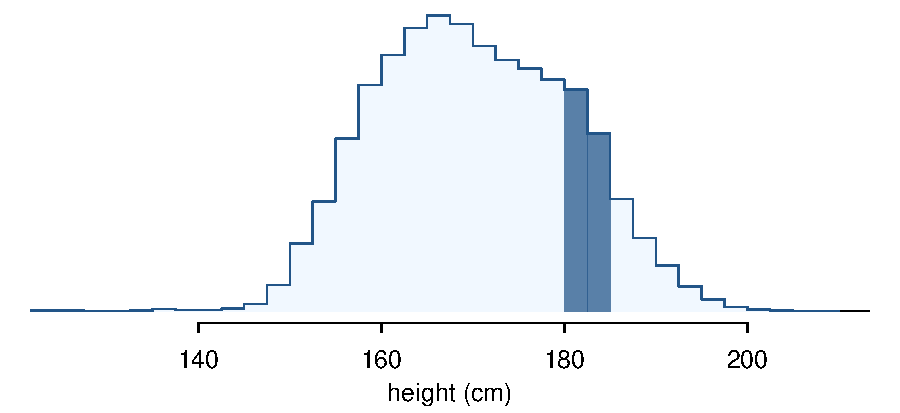
\includegraphics[width=\textwidth]{3-5_continuous_distributions/figures/usHeightsHist180185/usHeightsHist180185}
\end{center}


\end{frame}

%%%%%%%%%%%%%%%%%%%%%%%%%%%%%%%%%%%%

\subsection{From histograms to continuous distributions}

\begin{frame}
\frametitle{From histograms to continuous distributions}

Since height is a continuous numerical variable, its \hl{probability density function} is a smooth curve.

\begin{center}
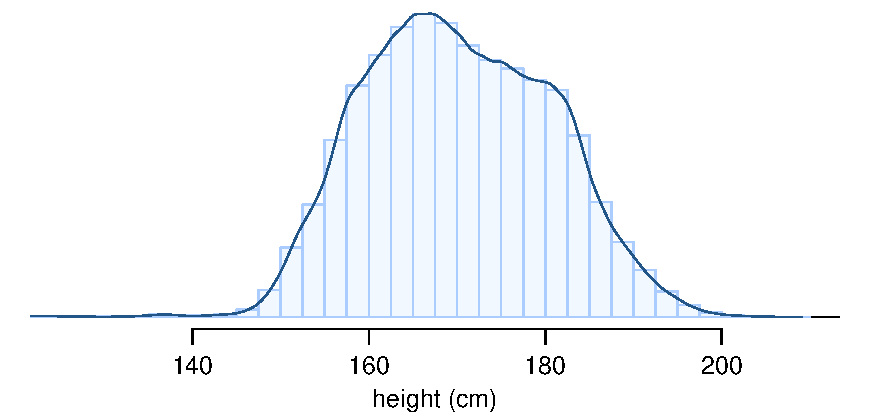
\includegraphics[width=\textwidth]{3-5_continuous_distributions/figures/fdicHeightContDist/fdicHeightContDist}
\end{center}

\end{frame}

%%%%%%%%%%%%%%%%%%%%%%%%%%%%%%%%%%%%

\subsection{Probabilities from continuous distributions}

\begin{frame}
\frametitle{Probabilities from continuous distributions}

Therefore, the probability that a randomly sampled US adult is between 180 cm and 185 cm can also be estimated as the shaded area under the curve.

\begin{center}
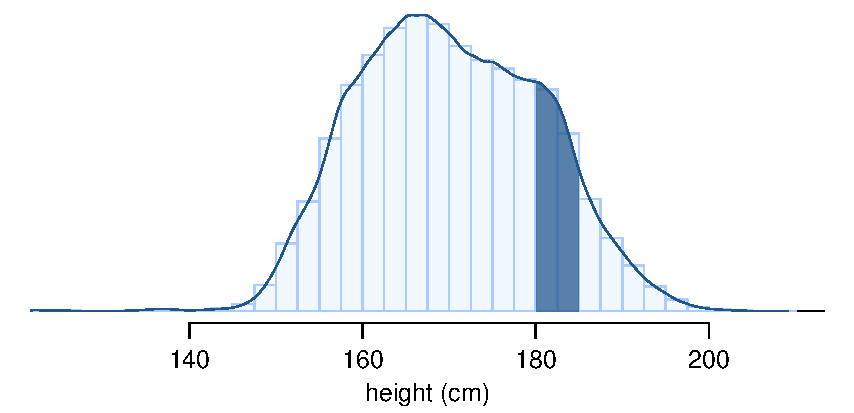
\includegraphics[width=\textwidth]{3-5_continuous_distributions/figures/fdicHeightContDistFilled/fdicHeightContDistFilled}
\end{center}


\end{frame}

%%%%%%%%%%%%%%%%%%%%%%%%%%%%%%%%%%%%

\begin{frame}
\frametitle{By definition...}

Since continuous probabilities are estimated as ``the area under the curve", the probability of a person being exactly 180 cm (or any exact value) is defined as 0.

\begin{center}
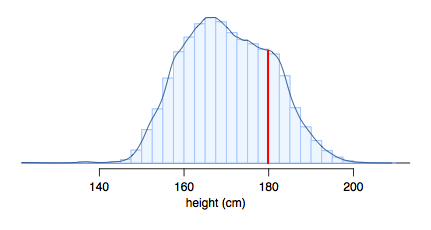
\includegraphics[width=0.8\textwidth]{3-5_continuous_distributions/figures/fdicHeightContDist180}
\end{center}

\end{frame}

%%%%%%%%%%%%%%%%%%%%%%%%%%%%%%%%%%%%

